% AI辅助说明：DeepSeek-V4-Pro，v4，DeepSeek，2026-08-30，
% 生成/辅助内容：论文主 LaTeX 文件结构、宏包配置、页眉页脚设置。
% 该内容经作者核对修改后用于复赛 B 题参赛论文。

\documentclass[12pt,a4paper]{ctexart}

% ============ 页面布局 ============
\usepackage[top=2.5cm, bottom=2.5cm, left=2.5cm, right=2.5cm, headheight=14.5pt]{geometry}

% ============ 页眉页脚 ============
\usepackage{fancyhdr}
\usepackage{lastpage}
\pagestyle{fancy}
\fancyhf{}
\fancyhead[C]{TeamBDATA2600409 \quad page \thepage \ of \pageref{LastPage}}
\renewcommand{\headrulewidth}{0.4pt}
\cfoot{\thepage}

% ============ 数学 ============
\usepackage{amsmath,amssymb}

% ============ 图形与表格 ============
\usepackage{graphicx}
\usepackage{float}
\usepackage{booktabs}
\usepackage{multirow}
\usepackage{array}
\usepackage{caption}
\usepackage{subcaption}

% ============ 超链接 ============
\usepackage[colorlinks=true,linkcolor=blue,citecolor=blue,urlcolor=blue]{hyperref}

% ============ 参考文献 ============
\usepackage[numbers,sort&compress]{natbib}
\bibliographystyle{unsrtnat}

% ============ 其他 ============
\usepackage{enumitem}
\usepackage{setspace}
\onehalfspacing

% ============ 图表编号格式 ============
\numberwithin{figure}{section}
\numberwithin{table}{section}
\numberwithin{equation}{section}

% ============ 行间公式允许分页 ============
\allowdisplaybreaks

% ============ 元数据 ============
\title{从燃油到纯电：电动汽车消费者转型回归分析}
\author{TeamBDATA2600409}
\date{2026年8月30日}

\begin{document}

% ============ 摘要页（第1页）============
\maketitle
\thispagestyle{empty}
\begin{abstract}
本道题目数据集为 50,000 条电动汽车消费者记录，三个子任务分别为对用户月度能源消耗量、月度充电成本与燃油替代支出的回归预测，评分指标为调整决定系数（adj-$R^2$）。

本题难点在于数据维度较高（23 列）、目标间存在级联关系，且题面提示的车型交互、复杂非线性等方向具有较强的误导性。在数据探索阶段，本文通过比率诊断与相关分析，识别出数据背后近似确定性的生成机制：能耗与周行驶里程成比例、燃油支出与日通勤里程成比例、充电成本近似等于能耗与电价的乘积。据此，本文并未采用复杂模型，而是以稀疏的物理公式与线性模型作为主方案。

在子任务一中，本文以周里程比率均值模型预测月度能耗，得到 adj-$R^2=0.876298$。在子任务二中，本文设计严格嵌套 OOF 级联方案，以任务一的折外预测乘以电价预测充电成本，得到 adj-$R^2=0.917817$，并给出真实能耗下的理论上界 0.9994。在子任务三中，本文以日通勤过原点 OLS 预测燃油支出，得到 adj-$R^2=0.905416$。

进一步的消融与残差诊断表明，题面建议的车型交互特征无增益，浅层 LightGBM 残差模型在 Bootstrap 置信区间下全面劣于稀疏基线，验证了``物理结构优先、复杂模型克制''的建模思路。本文的负结果报告为同类合成数据竞赛提供了可复用的方法学模板。

本文所有代码和中间文件均在支撑材料中随论文提交，并在 GitHub 仓库 \url{https://github.com/blackwhitetony/innoCupTaskB_Rematch} 中开源。核心实验均可在 CPU 上于数十秒内复现。

\textbf{关键词：}电动汽车 回归预测 稀疏物理模型 嵌套交叉验证 调整决定系数
\end{abstract}


% ============ 目录页（第2页起）============
\newpage
\pagestyle{empty}
\tableofcontents
\newpage

% ============ 正文开始（第3页起，页码从1开始）============
\setcounter{page}{1}
\pagestyle{fancy}

\section{问题背景与重述}

\subsection{赛题背景}

电动汽车正在重塑交通的未来。电力公司需要预测电动汽车接入电网后的负荷，金融机构需要评估用户的用车经济压力，政策制定者则需要量化用户从燃油车转向电动车后所节省的潜在支出。这三类诉求分别对应消费者转型过程中的三个关键经济变量：月度能源消耗量、月度充电成本与燃油替代支出。《电动汽车革命：消费者行为与充电洞察》数据集收录 50,000 条消费者记录，涵盖人口统计、通勤行为、充电基础设施、环保意识、技术接受度及财务等维度，为上述三类预测提供了信息基础。

\subsection{三个子问题}

赛题的核心是三个回归任务。它们的预测目标与评分指标汇总在表\ref{tab:tasks}中。

\begin{table}[H]
\centering
\caption{赛题子问题概览}
\label{tab:tasks}
\begin{tabular}{cccc}
\toprule
\textbf{子问题} & \textbf{预测目标} & \textbf{类型} & \textbf{评分指标} \\
\midrule
任务一：月度能源消耗量预测 & monthly\_energy\_consumption\_kwh & 回归 & adj-$R^2$ \\
任务二：月度充电成本预测 & monthly\_charging\_cost & 回归 & adj-$R^2$ \\
任务三：燃油替代支出预测 & fuel\_expense\_per\_month & 回归 & adj-$R^2$ \\
\bottomrule
\end{tabular}
\end{table}

三个子问题共用同一份数据，但目标之间存在级联关系：月度充电成本在物理上近似等于月度能耗与电价的乘积，因此任务二的建模结果直接依赖任务一的预测精度。此外，任务三要求基于用户当前的出行习惯与车辆属性，预测其若继续驾驶燃油车的月度燃油支出，属于反事实推断。

\subsection{总体技术路线}

为保证结果可复现且不同方案之间具备可比性，三项任务共用一套实验框架：

\begin{enumerate}[itemsep=0pt]
\item 首先进行数据 Schema 校验与固定折划分：使用固定随机种子生成 5 折划分，并额外生成 3 组随机种子（42/2026/7）用于最终确认；
\item 所有数据变换（缺失值填补、编码器、缩尾边界）仅在训练折内部拟合，禁止利用验证折或测试集统计量；
\item 每项任务先以可解释的物理公式或线性模型建立稀疏基线，再通过特征块消融与残差诊断判断是否引入非线性模型；
\item 复杂模型仅在越过预设晋级门槛（OOF adj-$R^2$ 增益 $\ge 0.0002$ 且 Bootstrap 95\% 区间下界大于 0）时采用；
\item 模型确定后，在 5 折 $\times$ 3 种子上仅做一次最终确认，不再反复调整。
\end{enumerate}

本研究的核心原则是``物理结构优先、复杂模型克制''：当数据本身可由近似确定性的公式刻画时，稀疏模型不仅可解释性更强，且在调整决定系数的评分口径下更具优势——因为每增加一个无增益的预测变量都会带来自由度惩罚。

\section{数据探索与预处理}

\subsection{数据概况}

原始数据集共 50,000 条记录，包含 23 个字段。其中 4 个分类变量（education\_level、city\_type、current\_vehicle\_type、ev\_adoption\_likelihood）、2 个二值变量（home\_charging\_available、previous\_ev\_experience）、14 个连续数值变量，以及 3 个目标变量（monthly\_energy\_consumption\_kwh、monthly\_charging\_cost、fuel\_expense\_per\_month）。

数据质量总体良好：无重复行、无无穷值、无常量列。存在三处缺失：education\_level、charging\_station\_accessibility、ev\_knowledge\_score 各缺失 500 条（各占 1\%），缺失模式近似随机。另有两处值得注意的分布特征：fuel\_expense\_per\_month 存在 271 个负值（最小值 $-99.7$），属业务语义上的异常；electricity\_cost\_per\_kwh 范围为 0.08--0.35，共 28 个离散取值。

三个任务的目标变量分布如表\ref{tab:target_dist}所示。

\begin{table}[H]
\centering
\caption{目标变量分布}
\label{tab:target_dist}
\begin{tabular}{ccccc}
\toprule
\textbf{任务} & \textbf{目标} & \textbf{均值 $\pm$ 标准差} & \textbf{范围} & \textbf{偏度} \\
\midrule
任务一 & 月能耗 & $186.74 \pm 88.25$ & 15.6--645.9 & 0.539 \\
任务二 & 充电成本 & $40.24 \pm 24.94$ & 1.4--199.6 & 1.067 \\
任务三 & 燃油支出 & $295.17 \pm 130.18$ & $-99.7$--862.0 & 0.104 \\
\bottomrule
\end{tabular}
\end{table}

\subsection{数据生成机制识别}

在进入建模之前，本文首先通过比率诊断与相关分析，识别数据背后近似确定性的生成机制。这一``先结构、后模型''的思路贯穿全文。

\subsubsection{核心相关性}

如图\ref{fig:corr}所示，三个目标与对应的出行变量之间存在极强的线性关系：月能耗与周里程的 Pearson 相关系数为 0.936，燃油支出与日通勤里程的相关系数为 0.952，充电成本同时受月能耗（0.765）与电价（0.584）驱动。这一相关性结构为后续的稀疏建模提供了直接依据。

\begin{figure}[H]
\centering
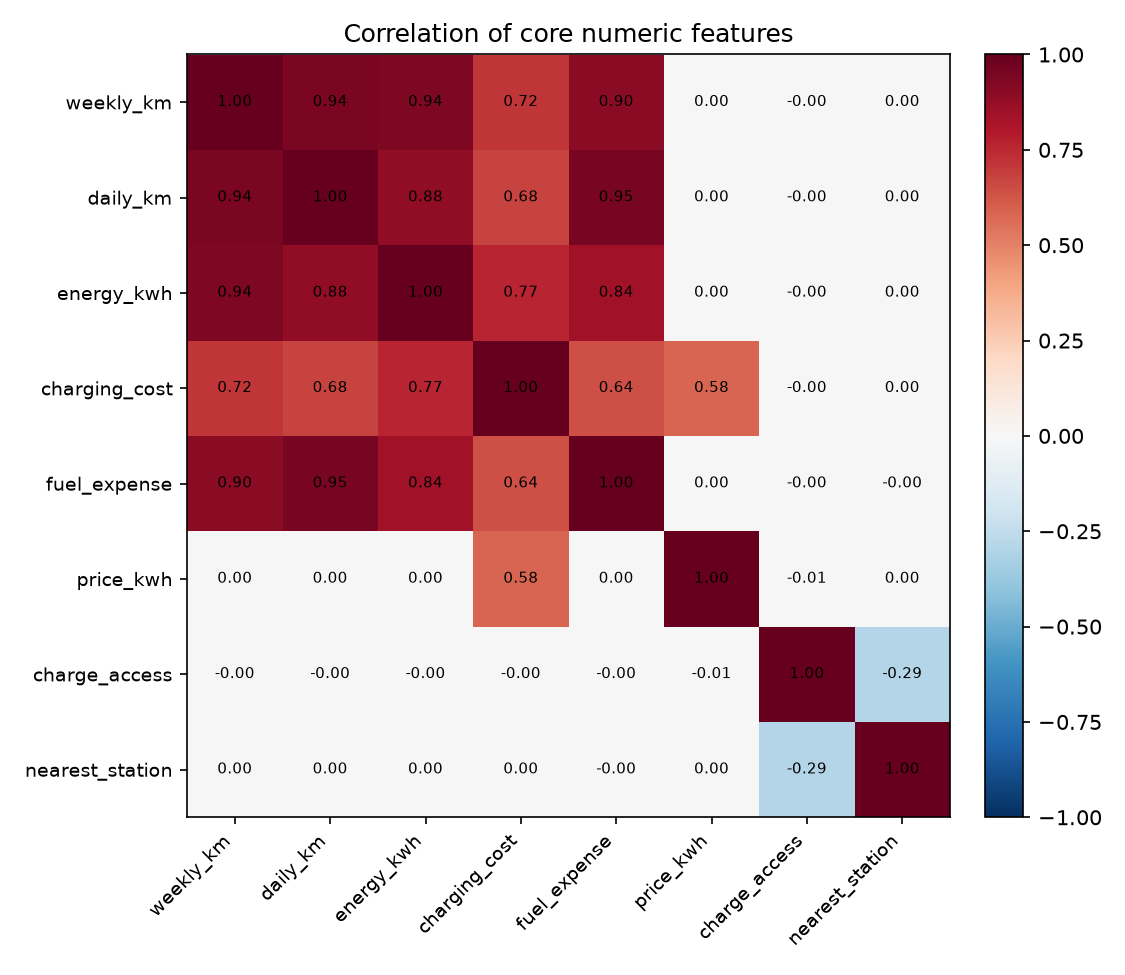
\includegraphics[width=0.85\textwidth]{figures/correlation_heatmap.png}
\caption{核心数值特征相关性热力图}
\label{fig:corr}
\end{figure}

\subsubsection{比率诊断}

进一步，本文考察若干关键比率变量的分布，以验证其是否服从某种随机生成机制：

\begin{enumerate}[itemsep=0pt]
\item \textbf{周里程/日通勤}：均值 6.50、标准差 0.87，与均匀分布 $U(5,8)$ 的理论均值（6.5）与标准差（0.866）高度吻合，表明周里程约为日通勤的 5--8 倍随机倍数；
\item \textbf{月能耗/周里程}：均值 0.816、范围 0.60--1.03，近似一个与其余特征无关的随机量，说明周里程是能耗的核心驱动变量；
\item \textbf{燃油支出/日通勤}：拟合过原点 OLS 得系数 8.395，残差标准差约 40，与公式 $fuel \approx 8.4 \times daily + N(0,40^2)$ 一致；
\item \textbf{充电成本/(能耗 $\times$ 电价)}：以能耗与电价的乘积预测成本，得到 $R^2=0.9994$，说明充电成本几乎由该乘积完全确定。
\end{enumerate}

上述机制意味着：题面提示的车型交互、地域差异等复杂映射在当前数据中并不存在，简单模型反而更贴近真实的数据结构。

\subsection{数据清洗流水线}

完整预处理流程由单一 Python 脚本实现，全链路可复现。步骤如下：

\begin{enumerate}[itemsep=0pt]
\item \textbf{Schema 校验}：每次训练前自动检查文件 SHA-256、行数、列名与顺序、类型、目标存在性、重复行、缺失、无穷值、非法类别与数值边界，结果写入 JSON 报告；
\item \textbf{固定折划分}：以随机种子 42/2026/7 生成 3 组 5 折划分，三任务共用同一组 fold\_id，保证跨任务可比与可复现；
\item \textbf{分类缺失值填充}：education\_level 的 500 个缺失位置以字符串``Missing''填充，作为独立类别参与建模；
\item \textbf{数值缺失值填补}：charging\_station\_accessibility 与 ev\_knowledge\_score 以训练折中位数填补（折内拟合，验证折只应用）；
\item \textbf{异常值处理}：fuel\_expense\_per\_month 的 271 个负值予以保留，不做截断或对数变换——这一决策由消融实验支撑（详见任务三）；
\item \textbf{编码}：线性模型对分类变量做 One-Hot（drop first），数值列标准化；树模型保留类别 dtype 与原生缺失处理。
\end{enumerate}

\subsection{最终数据规格}

清洗后数据保持 50,000 行，特征矩阵在 One-Hot 编码后为 27 维（14 个标准化数值列 + 11 个 One-Hot 列 + 2 个二值列）。三项任务的建模均以该流水线为统一入口，所有填补与编码均在交叉验证的折内完成，杜绝信息泄漏。

\section{子问题一：月度能源消耗量预测}

\subsection{问题定义与难点}

任务一的目标是基于消费者的出行与车辆特征，预测其每月的电动汽车能源消耗量 monthly\_energy\_consumption\_kwh。电力公司可据此预测电动汽车接入电网后的负荷。评分指标为调整决定系数 adj-$R^2$。

题面提示的核心难点是``该指标与行驶距离强相关，但受驾驶习惯和车型影响，需挖掘 daily\_commute\_km 与 vehicle\_type 的交互特征''。然而，数据探索阶段的比率诊断已表明，月能耗与周里程之间近似比例关系，且``单位里程能耗''这一随机量几乎不随车型或驾驶习惯变化。

\subsection{探索性数据分析}

\subsubsection{周里程与能耗的线性关系}

如图\ref{fig:t1_scatter}所示，月能耗随周里程线性增长，散点沿一条通过原点的直线均匀分布。以周里程的比率均值模型（$energy = r \cdot weekly$，其中 $r = \mathrm{mean}(energy/weekly)$）拟合，折外 adj-$R^2$ 即达 0.876300。

\begin{figure}[H]
\centering
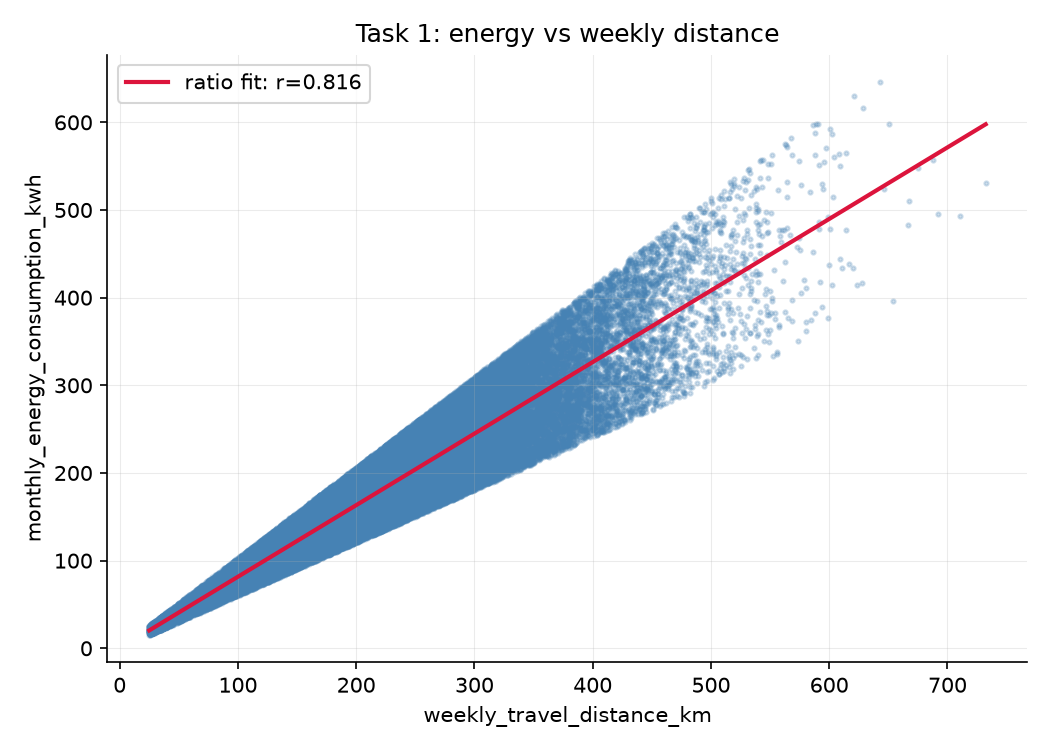
\includegraphics[width=0.8\textwidth]{figures/task1_energy_scatter.png}
\caption{月能耗与周行驶里程散点图及比率拟合线}
\label{fig:t1_scatter}
\end{figure}

\subsubsection{单位里程能耗的分布}

图\ref{fig:t1_ratio}给出单位里程能耗 $energy/weekly$ 的分布，近似为 0.60--1.03 区间内的平坦分布。该比率与所有可观测输入的相关系数绝对值均低于 0.01，各车型的平均值差异不足 0.001。这说明``能效''在当前数据中是一个与特征无关的随机量，模型能够解释的部分几乎全部来自周里程本身。

\begin{figure}[H]
\centering
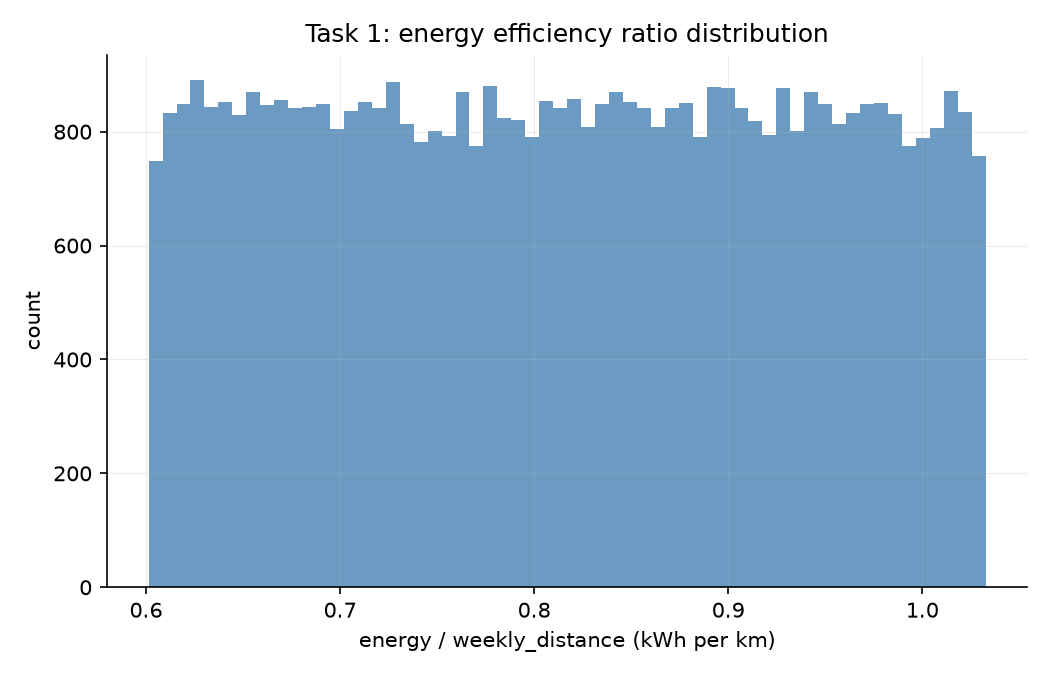
\includegraphics[width=0.8\textwidth]{figures/task1_ratio_dist.png}
\caption{单位里程能耗比率分布}
\label{fig:t1_ratio}
\end{figure}

\subsection{模型选择与消融}

\subsubsection{稀疏基线对比}

任务一首先比较三种稀疏基线：比率均值模型、过原点 OLS、带截距 OLS。结果如表\ref{tab:t1_baseline}所示，三者性能几乎一致，比率均值模型以 adj-$R^2=0.876300$ 略优，且具有最强的业务解释力。

\begin{table}[H]
\centering
\caption{任务一稀疏基线对比（5 折 OOF）}
\label{tab:t1_baseline}
\begin{tabular}{lccc}
\toprule
\textbf{模型} & \textbf{$R^2$} & \textbf{adj-$R^2$} & \textbf{RMSE} \\
\midrule
比率均值（$r\cdot weekly$） & 0.876302 & \textbf{0.876300} & 31.04 \\
过原点 OLS & 0.876296 & 0.876293 & 31.04 \\
带截距 OLS & 0.876290 & 0.876288 & 31.04 \\
\bottomrule
\end{tabular}
\end{table}

\subsubsection{特征块消融}

本文进一步验证题面建议的特征方向是否有效。以周里程为核心，逐块加入行程结构、官方车型交互、车辆/地域与其他信息特征，结果如表\ref{tab:t1_ablation}所示。

\begin{table}[H]
\centering
\caption{任务一特征块消融结果（adj-$R^2$）}
\label{tab:t1_ablation}
\begin{tabular}{lcc}
\toprule
\textbf{特征组合} & \textbf{特征数} & \textbf{adj-$R^2$} \\
\midrule
F0 核心（周里程） & 1 & \textbf{0.876300} \\
F0 + 行程结构 & 4 & 0.876277 \\
F0 + 官方车型交互 & 7 & 0.876271 \\
F0 + 车辆/地域 & 7 & 0.876244 \\
F0 + 其他信息 & 20 & 0.876198 \\
全特征 & 35 & 0.876149 \\
\bottomrule
\end{tabular}
\end{table}

消融结果与数据生成机制完全一致：任何特征块的加入都使 adj-$R^2$ 下降，官方提示的``里程 $\times$ 车型''交互无任何增益。原因在于 adj-$R^2$ 对新增预测变量施加自由度惩罚，而无增益特征只会增加模型复杂度。最终模型确定为单变量比率均值模型。

\subsection{残差诊断与非线性确认}

为验证稀疏模型是否已充分拟合，本文在基线的折内残差上训练浅层 LightGBM，观察其能否解释残差中的剩余结构。结果如表\ref{tab:t1_tree}所示：树模型相对基线的 $\Delta R^2$ 为 $-0.001430$，Bootstrap 95\% 置信区间为 $[-0.001799, -0.001070]$，整体小于 0。树模型不仅无增益，反而因拟合噪声而变差。

\begin{table}[H]
\centering
\caption{任务一树模型残差确认}
\label{tab:t1_tree}
\begin{tabular}{lccc}
\toprule
\textbf{方案} & \textbf{$R^2$} & \textbf{$\Delta R^2$（Bootstrap 95\% CI）} & \textbf{结论} \\
\midrule
稀疏基线 & 0.876300 & -- & 主方案 \\
残差 LightGBM & 0.874881 & $[-0.001799, -0.001070]$ & 淘汰 \\
\bottomrule
\end{tabular}
\end{table}

\subsection{最终模型}

任务一的最终模型为：

\begin{equation}
\hat{y}_1 = r_1 \cdot weekly\_travel\_distance\_km, \quad r_1 = 0.8163487
\label{eq:t1}
\end{equation}

在 5 折 $\times$ 3 种子最终确认中，adj-$R^2$ 均值为 0.876298 $\pm$ 0.000007，折间标准差极小，模型高度稳定。

\section{子问题二：月度充电成本预测}

\subsection{问题定义与难点}

任务二的目标是预测用户每月的充电总支出 monthly\_charging\_cost，金融机构可据此评估用户的用车经济压力。题面建议的输入特征包括 electricity\_cost\_per\_kwh、monthly\_energy\_consumption\_kwh（可用任务一的预测值作为级联特征）、fuel\_expense\_per\_month 等，并提示该问题``高度非线性''。

数据探索阶段的关键发现是：充电成本几乎等于月能耗与电价的乘积（$R^2=0.9994$）。因此本任务的难点并不在于拟合复杂的非线性关系，而在于如何在没有真实能耗的情况下，以无泄漏的方式构造级联预测。

\subsection{核心物理关系}

如图\ref{fig:t2_scatter}所示，monthly\_charging\_cost 与 ``monthly\_energy\_consumption\_kwh $\times$ electricity\_cost\_per\_kwh'' 几乎严格落在对角线 $y=x$ 上，全量数据拟合 $R^2=0.9994$、RMSE=0.60。这意味着充电成本由一个确定性公式刻画，唯一的建模空间在于能耗的预测精度。

\begin{figure}[H]
\centering
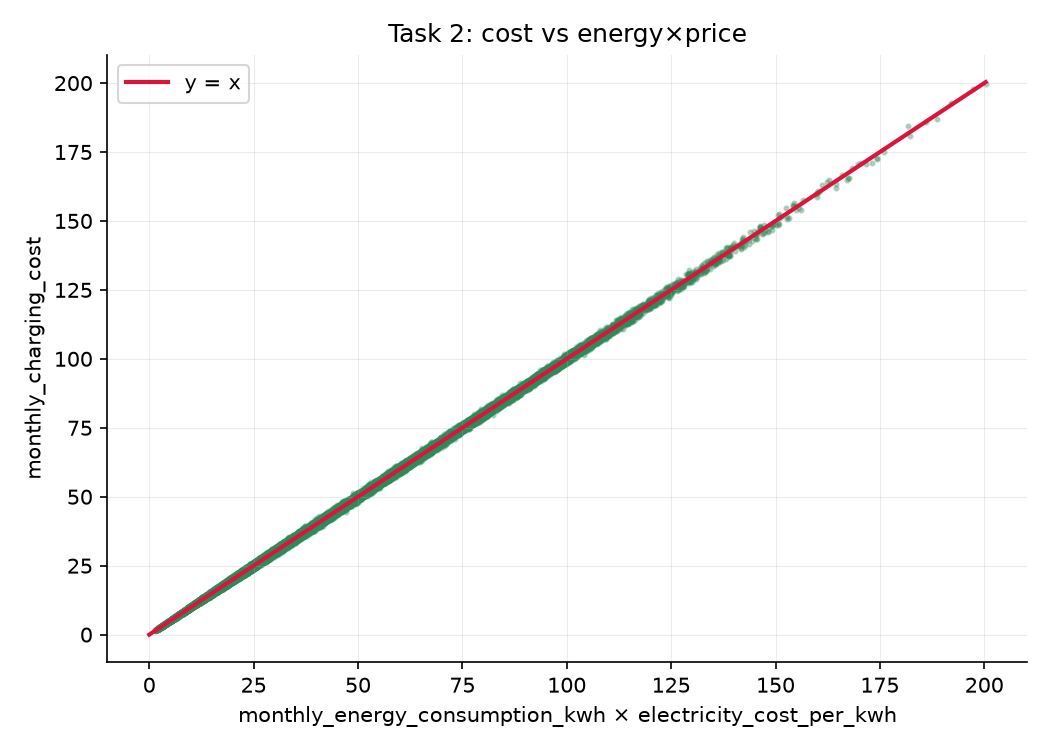
\includegraphics[width=0.8\textwidth]{figures/task2_cost_scatter.png}
\caption{充电成本与能耗$\times$电价的关系}
\label{fig:t2_scatter}
\end{figure}

\subsection{泄露边界与严格嵌套级联}

任务二的关键风险在于\textbf{teacher forcing}：如果在训练时使用真实能耗、而在测试时改用任务一的预测能耗，将造成训练与推理的分布错位，线下指标虚高而线上崩溃。为规避这一风险，本文设计了严格嵌套 OOF 级联方案：

\begin{enumerate}[itemsep=0pt]
\item 划分任务二的外层训练折 $A$ 与验证折 $B$；
\item 在 $A$ 内部再次交叉验证任务一，为 $A$ 中每行生成内层 OOF 能耗预测；
\item 用 $A$ 的全部数据重训任务一模型，预测 $B$ 的能耗；
\item 在 $A$ 上使用内层 OOF 能耗、在 $B$ 上使用外层预测能耗，分别构造 $\hat{cost} = \hat{energy} \times price$；
\item 汇总所有外层 $B$ 得到任务二的最终 OOF 预测。
\end{enumerate}

该方案从机制上保证了验证折的能耗预测从未见到验证折的真实能耗，杜绝了跨折信息传递。

\subsection{实验结果}

\subsubsection{方案对比}

任务二的各方案对比如表\ref{tab:t2_results}所示。

\begin{table}[H]
\centering
\caption{任务二方案对比（5 折 OOF）}
\label{tab:t2_results}
\begin{tabular}{lccc}
\toprule
\textbf{方案} & \textbf{$R^2$} & \textbf{adj-$R^2$} & \textbf{说明} \\
\midrule
严格嵌套级联（$\hat{energy}\times price$） & \textbf{0.917824} & \textbf{0.917820} & 主方案 \\
无级联 Ridge（周里程+日通勤+电价） & 0.851358 & 0.851349 & 对比基线 \\
真实能耗 $\times$ 电价 & 0.999428 & 0.999428 & Oracle 上界 \\
\bottomrule
\end{tabular}
\end{table}

严格嵌套级联方案得到 adj-$R^2=0.917820$，显著优于不依赖级联的对比基线（0.851358）。Oracle 方案（0.999428）说明，若测试时提供真实能耗，理论上界接近 1；但该值仅作诊断参照，不参与排名。

\subsubsection{级联后的进一步建模}

本文进一步检验：在级联特征 $\hat{cost} = \hat{energy} \times price$ 之上做线性校准、或加入官方建议的燃油支出特征，能否带来增益。结果如表\ref{tab:t2_ablation}所示，两种做法均使 adj-$R^2$ 略有下降。

\begin{table}[H]
\centering
\caption{任务二级联后消融（adj-$R^2$）}
\label{tab:t2_ablation}
\begin{tabular}{lcc}
\toprule
\textbf{方案} & \textbf{特征数} & \textbf{adj-$R^2$} \\
\midrule
纯级联 $\hat{cost}$ & 2 & \textbf{0.917820} \\
级联 + 线性校准 & 3 & 0.917794 \\
级联 + 燃油支出特征 & 4 & 0.917791 \\
\bottomrule
\end{tabular}
\end{table}

这一结果表明，任务二的误差几乎全部来自任务一能耗预测的个体能效误差，而非成本映射本身；在级联之上叠加任何模型都只是增加自由度惩罚。

\subsection{最终模型}

任务二的最终模型为：

\begin{equation}
\hat{y}_2 = r_1 \cdot weekly\_travel\_distance\_km \cdot electricity\_cost\_per\_kwh
\label{eq:t2}
\end{equation}

其中 $r_1=0.8163487$ 复用任务一的比率系数。在 5 折 $\times$ 3 种子最终确认中，adj-$R^2$ 均值为 0.917817 $\pm$ 0.000004。

\section{子问题三：燃油替代支出预测}

\subsection{问题定义与难点}

任务三的目标是基于用户当前的出行习惯与车辆属性，预测其若继续驾驶燃油车每月需要承担的燃油支出 fuel\_expense\_per\_month。政策制定者可据此量化用户转型电动车的潜在节省金额。这是一个反事实推断问题，评分指标为 adj-$R^2$。

题面提示该任务``需理解车型+里程+地域对油价的复杂映射关系''。然而数据探索表明，燃油支出几乎由日通勤里程单变量决定（相关系数 0.952），并叠加一个标准差约 40 的加性噪声。

\subsection{探索性数据分析}

\subsubsection{日通勤与燃油支出的线性关系}

如图\ref{fig:t3_scatter}所示，燃油支出随日通勤里程线性增长。过原点 OLS 拟合得到系数 $\beta=8.395$，折外 adj-$R^2=0.905416$。

\begin{figure}[H]
\centering
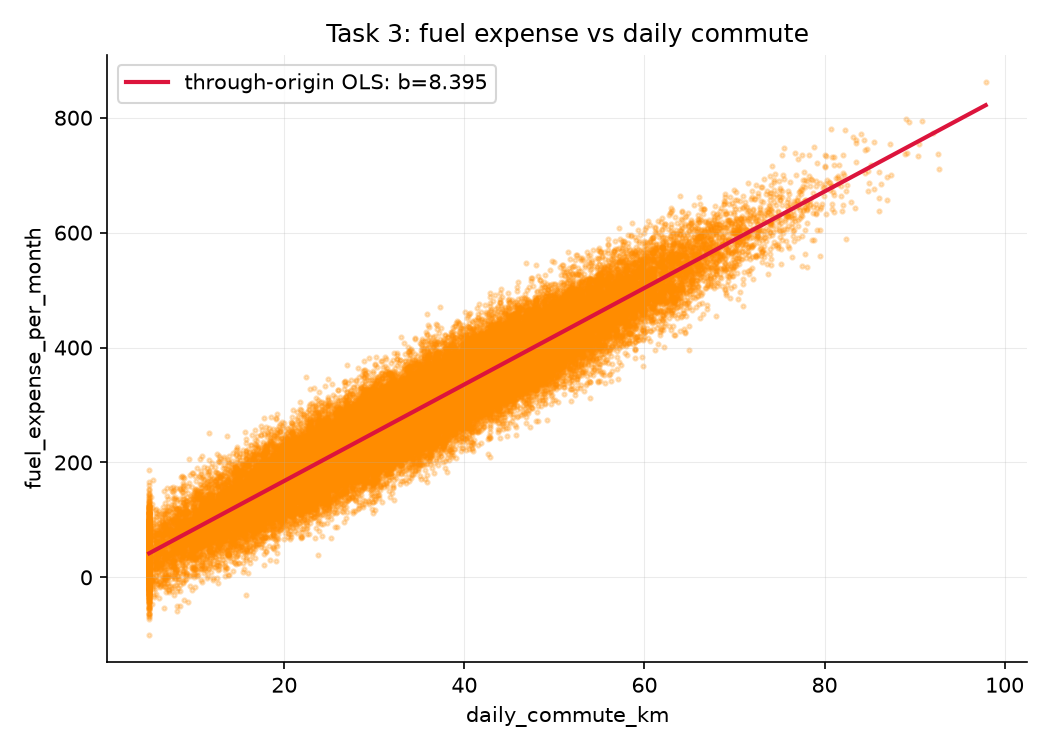
\includegraphics[width=0.8\textwidth]{figures/task3_fuel_scatter.png}
\caption{燃油支出与日通勤里程散点图及拟合线}
\label{fig:t3_scatter}
\end{figure}

\subsubsection{负值样本分布}

图\ref{fig:t3_dist}展示了燃油支出的分布，其中存在 271 个负值（最小值 $-99.7$），集中在低通勤区间。这些负值在业务语义上无效，但在统计上符合加性噪声的生成机制。

\begin{figure}[H]
\centering
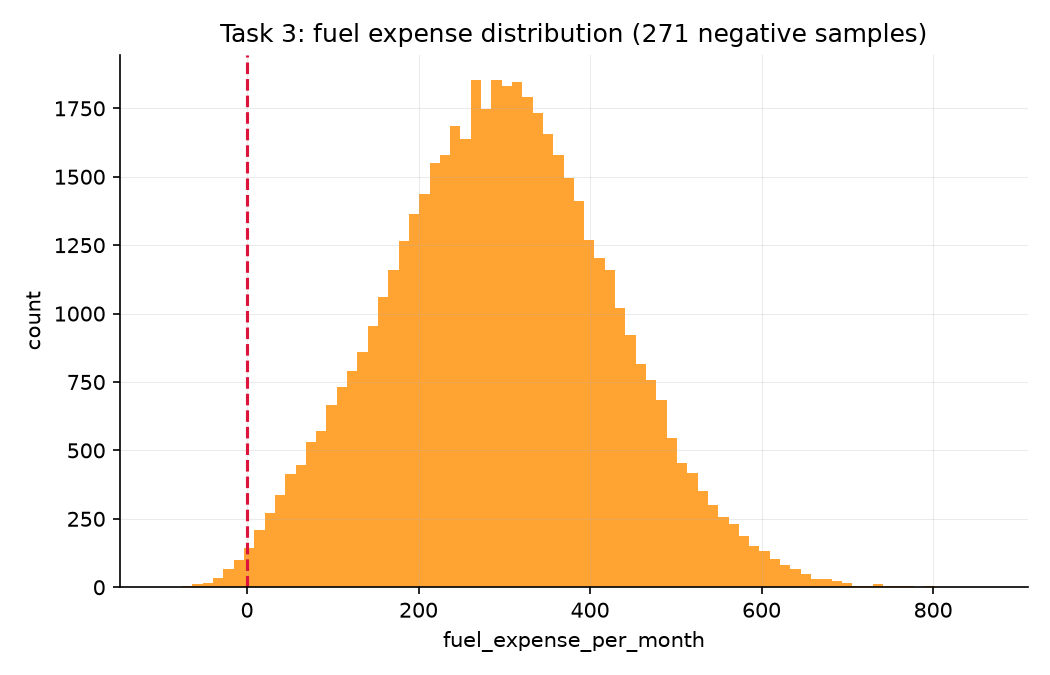
\includegraphics[width=0.8\textwidth]{figures/task3_target_dist.png}
\caption{燃油支出分布（含 271 个负值样本）}
\label{fig:t3_dist}
\end{figure}

\subsection{异常值处理策略}

针对负值样本，本文比较了四种处理策略：保留原值（过原点 OLS）、Huber 稳健回归、目标缩尾、删除负样本训练。结果如表\ref{tab:t3_outlier}所示。

\begin{table}[H]
\centering
\caption{任务三异常值处理策略对比（adj-$R^2$）}
\label{tab:t3_outlier}
\begin{tabular}{lcc}
\toprule
\textbf{策略} & \textbf{adj-$R^2$} & \textbf{说明} \\
\midrule
保留原值（过原点 OLS） & \textbf{0.905416} & 主方案 \\
Huber 稳健回归 & 0.905405 & 略降 \\
删除负样本训练 & 0.905369 & 略降 \\
目标缩尾（clip 到 $[0, Q_{99}]$） & 0.905280 & 明显下降 \\
\bottomrule
\end{tabular}
\end{table}

删除负值或对目标做缩尾、截断均使 adj-$R^2$ 下降，原因是负值样本与加性噪声结构一致，机械处理反而破坏了数据的真实分布。最终模型保留原始目标，不做对数变换与预测截断。

\subsection{特征块消融}

本文同样验证了题面建议的``车型+里程+地域''复杂映射是否有效。以日通勤为核心逐块加入特征，结果如表\ref{tab:t3_ablation}所示。

\begin{table}[H]
\centering
\caption{任务三特征块消融结果（adj-$R^2$）}
\label{tab:t3_ablation}
\begin{tabular}{lcc}
\toprule
\textbf{特征组合} & \textbf{特征数} & \textbf{adj-$R^2$} \\
\midrule
F0 核心（日通勤） & 1 & \textbf{0.905416} \\
F0 + 行程结构 & 4 & 0.905395 \\
F0 + 官方车型/地域交互 & 6 & 0.905374 \\
F0 + 车辆/地域 & 8 & 0.905379 \\
F0 + 其他信息 & 18 & 0.905371 \\
全特征 & 33 & 0.905311 \\
\bottomrule
\end{tabular}
\end{table}

与任务一一致，任何特征块的加入都无法提升 adj-$R^2$，官方提示的车型、地域交互在当前数据中不存在增益。

\subsection{残差诊断与非线性确认}

在日通勤过原点 OLS 的折内残差上训练浅层 LightGBM，其相对基线的 $\Delta R^2$ 为 $-0.000355$，Bootstrap 95\% 置信区间为 $[-0.000466, -0.000257]$，整体小于 0（表\ref{tab:t3_tree}）。树模型同样被淘汰。

\begin{table}[H]
\centering
\caption{任务三树模型残差确认}
\label{tab:t3_tree}
\begin{tabular}{lccc}
\toprule
\textbf{方案} & \textbf{$R^2$} & \textbf{$\Delta R^2$（Bootstrap 95\% CI）} & \textbf{结论} \\
\midrule
稀疏基线 & 0.905418 & -- & 主方案 \\
残差 LightGBM & 0.905056 & $[-0.000466, -0.000257]$ & 淘汰 \\
\bottomrule
\end{tabular}
\end{table}

\subsection{最终模型}

任务三的最终模型为：

\begin{equation}
\hat{y}_3 = \beta \cdot daily\_commute\_km, \quad \beta = 8.3947643
\label{eq:t3}
\end{equation}

在 5 折 $\times$ 3 种子最终确认中，adj-$R^2$ 均值为 0.905416 $\pm$ 0.000002。剩余约 40 的残差标准差接近不可约的加性噪声，说明在当前特征集合下模型已逼近预测上限。

\section{综合讨论}

\subsection{三任务横向对比}

三项任务共享同一数据集、同一预处理流水线与同一套验证框架，但呈现出高度一致的结构特征：稀疏物理公式即可逼近预测上限。表\ref{tab:overall}汇总了关键指标。

\begin{table}[H]
\centering
\caption{三项任务综合对比}
\label{tab:overall}
\begin{tabular}{lcccl}
\toprule
\textbf{维度} & \textbf{任务一} & \textbf{任务二} & \textbf{任务三} & \textbf{说明} \\
\midrule
核心驱动变量 & 周里程 & 能耗 $\times$ 电价 & 日通勤 & \\
最终模型 & 比率均值 & 级联公式 & 过原点 OLS & \\
adj-$R^2$ & 0.876298 & 0.917817 & 0.905416 & 5折$\times$3种子均值 \\
折间标准差 & 0.000007 & 0.000004 & 0.000002 & 高度稳定 \\
残差树模型 $\Delta R^2$ & $-0.001430$ & $-0.000922$ & $-0.000355$ & 全部为负 \\
特征块消融 & 全部下降 & 级联最优 & 全部下降 & 稀疏最优 \\
\bottomrule
\end{tabular}
\end{table}

三项任务的共同结论是：数据由近似确定性的物理关系生成，稀疏模型已达预测上限，复杂模型（浅层提升树）在 Bootstrap 置信区间下全面劣化。

\subsection{物理结构优先的方法论}

本研究与初赛阶段形成鲜明对照。初赛三任务均为分类，采用 CatBoost 统一建模并取得了较强的信号；而本次复赛的回归目标背后存在近似确定性的生成公式，此时任何数据驱动模型都难以超越对该公式的精确刻画。这一对照指向一个可推广的方法论原则：\textbf{在投入大规模模型搜索之前，先通过比率诊断与相关分析识别数据的底层结构}，结构存在时以公式/线性模型为主，仅在残差存在稳定信号时才引入非线性模型。

\subsection{调整决定系数下的稀疏性权衡}

复赛以 adj-$R^2$ 为评分指标，这与初赛的准确率存在本质差异：adj-$R^2$ 会对新增预测变量施加自由度惩罚。因此，一个无增益特征的加入，即使不改变 $R^2$，也会降低 adj-$R^2$。本文的消融实验反复印证了这一点：特征块越多，adj-$R^2$ 越低。在``特征越多越好''的惯性思维下，这一指标反而奖励了最简洁的模型，与本文发现的数据结构不谋而合。

\subsection{严格级联的防泄漏价值}

任务二的严格嵌套 OOF 级联是本文在方法论层面的核心贡献之一。若图省事直接在训练时使用真实能耗、测试时改用预测能耗，将造成 teacher forcing，线下指标虚高、线上无法复现。本文的嵌套方案从机制上保证了能耗预测与成本建模的信息隔离，可复用于任何``预测-再预测''的级联回归场景。

\subsection{负结果的方法论价值}

与初赛任务二类似，本文保留了完整的负结果记录：题面建议的车型/地域交互、浅层提升树模型均被证伪。这些负结果的意义在于：

\begin{enumerate}[itemsep=0pt]
\item 明确界定了``模型选择不当''与``数据结构本身简单''两种情况的边界；
\item 通过 Bootstrap 置信区间而非单次实验的偶然提升来判定模型取舍，避免了过度拟合噪声；
\item 为同类合成数据竞赛提供了一套``结构识别 $\to$ 稀疏基线 $\to$ 消融 $\to$ 残差诊断 $\to$ 最终确认''的可复用流程。
\end{enumerate}

\section{结论与展望}

\subsection{主要发现}

1. \textbf{任务一（月度能耗预测）}：数据探索识别出``能耗 $\propto$ 周里程''的比例结构，单位里程能耗近似与特征无关的随机量。最终以单变量比率均值模型 $energy = 0.81635 \times weekly$ 得到 adj-$R^2=0.876298$。题面建议的``里程 $\times$ 车型''交互与全特征模型均使 adj-$R^2$ 下降。

2. \textbf{任务二（月度充电成本预测）}：充电成本近似由 ``能耗 $\times$ 电价''完全确定（$R^2=0.9994$）。本文以严格嵌套 OOF 级联规避 teacher forcing，最终模型 $cost = 0.81635 \times weekly \times price$ 得到 adj-$R^2=0.917817$，显著优于无级联基线。

3. \textbf{任务三（燃油替代支出预测）}：燃油支出由日通勤里程单变量驱动，叠加标准差约 40 的加性噪声。最终以过原点 OLS $fuel = 8.39476 \times daily$ 得到 adj-$R^2=0.905416$。保留负值样本优于删除、缩尾与 Huber 稳健回归。

4. \textbf{复杂模型全面证伪}：三个任务的浅层 LightGBM 残差模型在 Bootstrap 95\% 置信区间下 $\Delta R^2$ 全部为负，题面提示的交互特征均无增益，验证了``物理结构优先、复杂模型克制''的建模思路。

\subsection{方法学贡献}

\begin{enumerate}[itemsep=0pt]
\item \textbf{数据生成机制识别}：通过比率诊断与相关分析，在建模前即识别出近似确定性的生成公式，为模型选择提供了直接依据；
\item \textbf{严格嵌套级联设计}：任务二的 T1$\to$T2 级联在训练折内部再次交叉验证生成 OOF 能耗，从机制上杜绝 teacher forcing；
\item \textbf{证据驱动的模型晋级门槛}：以 pooled OOF adj-$R^2$ 增益、Bootstrap 95\% 置信区间与多随机种子稳定性三重标准判定模型取舍，而非依赖单次实验的偶然提升；
\item \textbf{负结果的诚实报告}：完整记录交互特征与复杂模型被证伪的全过程，为同类问题提供可复用的信号验证模板。
\end{enumerate}

\subsection{局限性}

1. \textbf{口径依赖组委会确认}：adj-$R^2$ 中自由度 $p$ 的定义、正式测试集的字段是否隐藏三个目标列、T2 是否提供真实能耗等问题尚待组委会明确，本文采用最保守的严格口径。

2. \textbf{非线性模型覆盖有限}：本文仅以浅层 LightGBM 作为非线性代表进行残差诊断，未穷举全部可能模型。但从消融与 Bootstrap 结果看，数据结构本身不支持非线性增益，该局限不影响结论。

3. \textbf{公式外推性未知}：最终模型为闭式公式，其系数依赖当前训练集；若正式测试集的生成机制与训练集不同（例如新增了与能效相关的变量），模型的鲁棒性有待检验。

4. \textbf{业务可解释性的边界}：任务三的负值燃油支出样本虽在统计上应保留，但在业务上仍属异常，其处理方式需在报告中向评审说明。


% ============ 参考文献 ============
\bibliography{refs}

% ============ AI工具使用声明 ============
\section*{AI工具使用声明}
\nocite{deepseek2026,lightgbm2017}

本参赛队在研究过程中使用了以下人工智能工具作为辅助手段。所有AI生成的内容均经作者严格核对、修改和验证，其正确性、可靠性及学术规范性由本参赛队承担全部责任。核心建模、算法设计、代码实现、结果分析与结论由队员独立完成。

具体使用情况如下：

\begin{itemize}[itemsep=4pt]
\item \textbf{DeepSeek-V4-Pro（v4，DeepSeek）}：用于数据 Schema 校验与清洗流水线设计、探索性数据分析（EDA）可视化脚本生成、稀疏基线与消融实验代码编写、严格嵌套级联方案实现，以及论文 LaTeX 结构与部分章节草稿的辅助生成。使用日期：2026年8月30日。

\item \textbf{Opencode（DeepSeek-V4-Pro，v4）}：作为交互式 CLI 编程辅助工具，在代码生成、实验运行与论文撰写环节提供辅助。仅作辅助作用，所有AI生成的内容均经作者严格核对、修改和验证，其正确性、可靠性及学术规范性由本参赛队承担全部责任。核心建模、算法设计、代码实现、结果分析与结论由队员独立完成。使用日期：2026年8月30日。
\end{itemize}

各章节中凡由AI辅助生成并修改后采用的内容，均已在对应位置以脚注标注（注明工具名称、提示词原文、生成日期及用途）。

本参赛队保证：全文AIGC生成比例不超过30\%，论文整体相似比不超过50\%。支撑材料中附有《AI工具使用详情说明》（文件名：BDATA2600409\_AI使用说明.pdf），包含工具基本信息、使用目的、关键交互记录及采纳修改说明。


% ============ 附录 ============
\appendix
\section{源代码文件清单}

本研究所使用的源代码文件如下（完整代码见支撑材料）：

\begin{table}[H]
\centering
\begin{tabular}{lp{7cm}}
\toprule
\textbf{文件} & \textbf{功能说明} \\
\midrule
src/schema\_check.py & Schema 校验：文件哈希、列名顺序、类型、缺失、重复、无穷、非法类别与边界 \\
src/preprocessing.py & 预处理模块：折内填补（中位数/Missing）、One-Hot 编码、标准化 \\
src/features.py & 特征矩阵构建与各任务特征块定义 \\
src/folds.py & 固定折划分（5 折 $\times$ 3 种子） \\
src/metrics.py & $R^2$、adj-$R^2$、RMSE、MAE 指标 \\
src/experiments.py & P2 稀疏基线 + P3 特征消融 + T2 严格嵌套级联 \\
src/finalize.py & P4 树模型残差确认 + P6 5折$\times$3种子最终确认 \\
src/submit.py & 最终模型拟合与提交 CSV 生成 \\
src/make\_figures.py & 论文 EDA 配图生成 \\
configs/schema.yaml & 数据 Schema 定义（列顺序、类型、边界、预期缺失） \\
configs/leakage.yaml & 泄露边界冻结（各任务可用/禁用特征清单） \\
\bottomrule
\end{tabular}
\end{table}

\section{运行环境}

\begin{table}[H]
\centering
\begin{tabular}{ll}
\toprule
\textbf{项目} & \textbf{配置} \\
\midrule
Python 版本 & 3.11 \\
包管理器 & uv \\
核心依赖 & scikit-learn, lightgbm, catboost, xgboost, pandas, numpy, matplotlib \\
算力 & CPU（无需 GPU） \\
操作系统 & Windows 11 \\
随机种子 & 42 / 2026 / 7 \\
\bottomrule
\end{tabular}
\end{table}

\section{开源代码仓库}

本项目全部代码、论文 LaTeX 源码及 EDA 配图均在 GitHub 平台开源：

\begin{itemize}[itemsep=2pt]
\item \textbf{仓库地址}：\url{https://github.com/blackwhitetony/innoCupTaskB_Rematch}
\item \textbf{主要目录}：src/（数据校验、预处理、特征、基线/消融、最终确认与提交脚本）、configs/（Schema 与泄露边界）、autodl/（在线平台复现脚本）、paper/（论文 LaTeX 源码）、reports/（结果摘要与方法论笔记）
\item \textbf{说明}：数据 CSV 不随仓库提交，复现时需自行将赛题数据置于 \texttt{复赛B题/B题数据集.csv}。
\end{itemize}

\section{模型调用方式}

最终模型均为闭式公式，参数存档于 artifacts/models/final\_models.json：

\begin{verbatim}
T1: energy = 0.8163487 * weekly_travel_distance_km
T2: cost   = 0.8163487 * weekly_travel_distance_km * electricity_cost_per_kwh
T3: fuel   = 8.3947643 * daily_commute_km
\end{verbatim}

支撑材料解压后，在项目根目录执行：

\begin{verbatim}
uv sync                          # 安装依赖
uv run python -m src.schema_check   # 数据校验
uv run python -m src.folds          # 生成固定折
uv run python -m src.experiments    # 基线 + 消融
uv run python -m src.finalize       # 残差确认 + 最终确认
uv run python -m src.submit         # 拟合最终模型 + 生成提交
\end{verbatim}

正式测试集到达后，执行 \texttt{uv run python -m src.submit --test <测试.csv>} 即可生成三份提交文件（T1/T2/T3），格式为 \texttt{row\_id, true, prediction}。


\end{document}
